\documentclass[twocolumn]{aastex701}
\usepackage{graphicx} % Required for inserting images
\usepackage{indentfirst}
\usepackage{amsmath, amssymb}
\usepackage{enumitem}
\begin{document}

\title{X-ray Characterization of Aerogel Foams: Quantifying When Scattering Effects Require Corrections for Accurate Density Measurement}

\author{Yuegelica Yeong, Pawel M. Kozlowski}
\affiliation{Institute for Computing in Research}
\email[show]{yuegelicay@gmail.com}

\begin{abstract}
Aerogel foams are known for their extremely high porosity and are increasingly utilized in high energy density (HED) physics experiments to study laser-driven radiative flows. These foams are optimal materials to study radiation flows due to their low and manipulable density. X-ray absorption imaging is a widely used technique to determine the density of these foams prior to experiments. However, it is typically assumed that the foam's attenuation follows the Beer-Lambert law, which neglects the presence of scattering. In this research project, we simulate X-rays at photon energies of 2, 5, and 8 keV through a cylindrical $(SiO_{2})_{5}+Ti$ foam with 1700 $\mu$m height and 900 $\mu$m diameter. We conducted statistical simulations to investigate when scattering effects become significant enough to impact density measurements. Specifically, we determine the conditions in which corrections to Beer-Lambert are necessary, using a threshold of $\pm 2$ mg/cc difference in density. We find that scattering effects grow with increasing porosity and pore size. We also found that refraction, but not increased path length, played an important role in causing significant scattering. This study determined the conditions when Beer-Lambert assumptions are valid, and when corrections are necessary for accurate aerogel characterization.
\end{abstract}

\keywords{X-ray imaging, aerogels, scattering, density measurement, high energy density physics}

\section{Introduction}

Aerogel foams, with their unique combination of ultra-low density and high porosity (typically 95-99.8\%), have become essential materials in high energy density (HED) physics experiments \citep{Lanier_Hamilton_Taccetti_2012}. These materials serve as targets in laser-driven experiments to study radiation transport, shock propagation, and astrophysical phenomena under controlled laboratory conditions. However, accurate pre-characterization of aerogel density remains a significant challenge that directly impacts experimental outcomes.

The conventional approach to aerogel density measurement relies on X-ray transmission imaging coupled with the Beer-Lambert law, which assumes pure absorption without scattering. This assumption works well for dense, homogeneous materials but may break down for highly porous aerogels where X-ray photons can undergo complex interactions with the foam microstructure. Recent observations have revealed systematic deviations in density measurements near aerogel edges, suggesting that scattering effects may be more significant than previously assumed.

\subsection{Motivation and Problem Statement}

Current density measurements of aerogel foams exhibit ``edge effects'' that cannot be explained by classical Beer-Lambert attenuation alone. While density measurements at the foam center appear reliable, measurements near the edges show significant deviations that may be attributed to X-ray scattering from the porous microstructure. This presents a critical problem for HED experiments, where precise knowledge of target density is essential for:

\begin{enumerate}
    \item Setting appropriate laser parameters and timing
    \item Predicting shock wave propagation speeds
    \item Interpreting diagnostic measurements
\end{enumerate}

The fundamental question addressed in this work is: \textit{Under what conditions do scattering effects become significant enough to require corrections to Beer-Lambert-based density measurements?}

\begin{figure}[t]
    \centering
    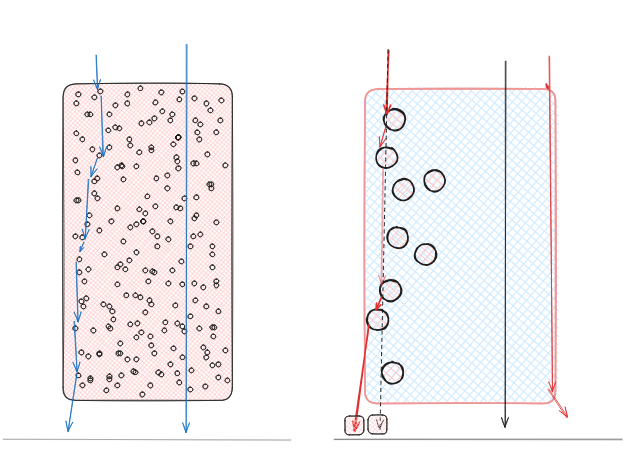
\includegraphics[width=0.35\linewidth]{sidebyside.png}
    \caption{Comparison of X-ray photon paths: (left) ideal Beer-Lambert attenuation assuming straight-line propagation, and (right) realistic attenuation including scattering effects that increase path length and cause lateral displacement.}
    \label{fig:side}
\end{figure}

\section{Background and Related Work}

\subsection{Aerogel Characterization Challenges}

Aerogel density characterization faces several fundamental challenges. The extremely low mass of typical aerogel samples (tens of micrograms) makes gravimetric measurements unreliable, with uncertainties often exceeding 7-8\% \citep{Lanier_Hamilton_Taccetti_2012}. Additionally, aerogels are inherently non-uniform materials, with density variations that can significantly impact local measurements.

Pre-characterization of foam properties is crucial because the foam is completely vaporized during HED experiments, making post-shot analysis impossible. Current density calibration systems, such as the Density Calibration Station (DCS), use X-ray absorption measurements combined with knowledge of foam thickness, composition, and X-ray energy to calculate density assuming pure absorption \citep{Johns_Fryer_Wood_Fontes_Kozlowski_Lanier_Liao_Perry_Morton_Brown_et_al._2021}.

\begin{figure}[t]
    \centering
    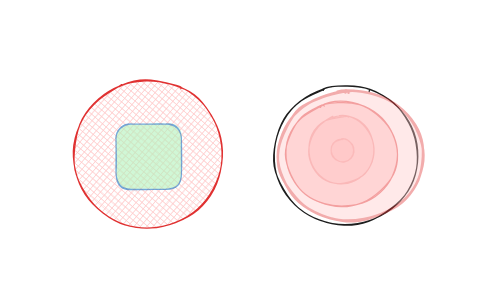
\includegraphics[width=0.45\linewidth]{circular.png}
    \caption{Schematic representation of X-ray transmission through aerogel foam. Beer-Lambert law provides accurate density measurements at the foam center, but edge effects become apparent near the boundaries due to scattering mechanisms.}
    \label{fig:circle}
\end{figure}

\subsection{HED Physics Applications}

Aerogel foams play a critical role in HED physics experiments designed to study radiation transport phenomena relevant to astrophysics and inertial confinement fusion. In these experiments, high-power lasers irradiate gold hohlraums, generating intense X-ray fields that drive radiation fronts through the aerogel targets. The foam composition, typically silica doped with metals such as titanium or scandium, is carefully chosen to provide specific opacity and temperature response characteristics.

The measured foam density directly determines the speed of radiation-driven shock waves and the resulting plasma conditions. Inaccurate density measurements can lead to misinterpretation of experimental results and poor agreement with theoretical predictions. Recent experimental campaigns such as COAX, Radishock, and Xflows have advanced our understanding of radiation transport in aerogels but have not systematically addressed the impact of X-ray scattering on density measurements \citep{Byvank_Coffing_Lioce_Fryer_Fontes_Kozlowski_Johns_Čamdžić_Elshafiey_Meyerhofer_et_al._2024, Fryer_Wood_Coffing_Robey_Fontes_Johns_Kozlowski_Urbatsch_Lanier_Meyerhofer_et_al._2023}.

\subsection{X-ray Scattering in Porous Materials}
X-ray interactions with porous materials involve several physical processes beyond simple photoelectric absorption. Sattering can deflect photons from their original trajectories, while refraction at pore interfaces can cause additional path deviations. For highly porous materials like aerogels, these effects may become significant enough to impact transmission measurements.

Previous studies of X-ray scattering in porous materials have primarily focused on geological samples or industrial foams with much lower porosity than aerogel targets used in HED experiments. The extreme porosity (>95$\%$) and nanoscale pore structure of aerogels represent a unique regime where traditional scattering approximations may not apply.

\subsection{COAX and Advanced Diagnostic Platforms}

The COAX platform, deployed on the OMEGA-60 laser facility, represents the current state-of-the-art for studying radiation transport in aerogel foams \citep{Byvank_Coffing_Lioce_Fryer_Fontes_Kozlowski_Johns_Čamdžić_Elshafiey_Meyerhofer_et_al._2024}. This diagnostic platform uses absorption spectroscopy and radiography to map foam temperature and density during radiation flow, enabling classification of supersonic, transonic, and subsonic flow regimes.

\begin{figure}[t]
    \centering
    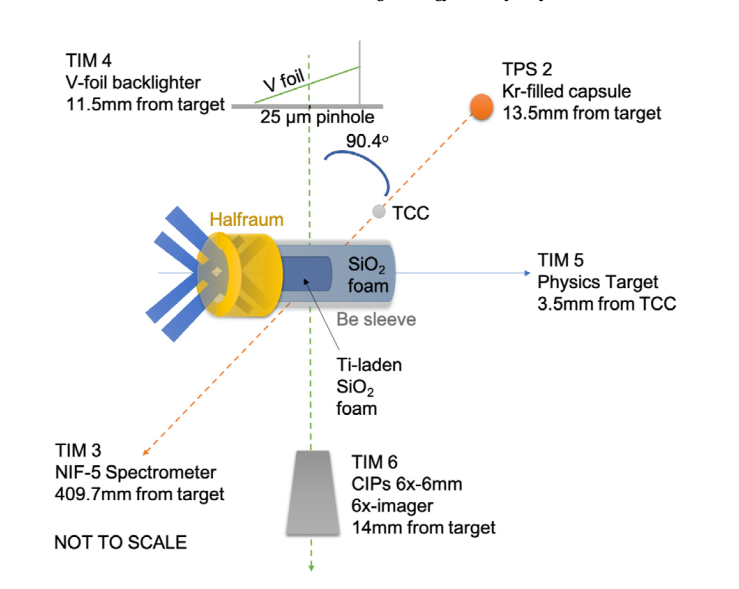
\includegraphics[width=0.45\linewidth]{coaxplatform.png}
    \caption{COAX platform configuration on the OMEGA-60 laser facility, showing the experimental setup used for studying radiation transport in titanium-doped silica aerogel foams.}
    \label{fig:coaxplatform}
\end{figure}

While these experiments have provided valuable insights into radiation transport physics, they have not quantitatively addressed how X-ray scattering during pre-shot characterization might affect the accuracy of initial density measurements. The Xflows experiments developed for the National Ignition Facility (NIF) have scaled up these techniques to achieve higher temperatures and longer radiation transport distances \citep{Johns_Byvank_Robey_Urbatsch_Coffing_Fryer_Perry_Kozlowski_Fontes_Love_et_al._2023}, but the fundamental scattering question remains unresolved.

\section{Methods and Simulations}

\subsection{Theoretical Framework}

Our simulation approach combines classical X-ray attenuation theory with statistical modeling of scattering processes in porous media. The foundation of our analysis rests on the Beer-Lambert law for X-ray attenuation:

\begin{equation}
\label{eq:BL Law}
    T = \frac{I}{I_0} = e^{-\mu \ell}
\end{equation}

where $T$ is the transmission coefficient, $I$ and $I_0$ are the transmitted and incident intensities respectively, $\mu$ is the linear attenuation coefficient, and $\ell$ is the effective path length through the material.

\begin{figure}[t]
    \centering
    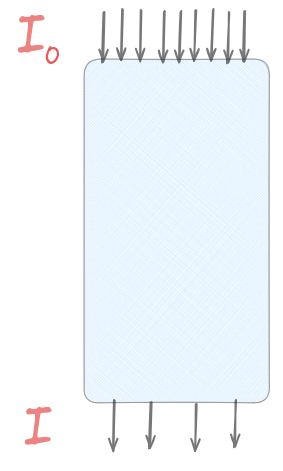
\includegraphics[width=0.45\linewidth]{intensity.png}
    \caption{Illustration of transmission calculation: with incident intensity $I_0 = 9$ and transmitted intensity $I = 4$, the transmission coefficient is $T = 4/9 \approx 0.44$.}
    \label{fig:nntensity}
\end{figure}

The key assumption of Beer-Lambert law is that photons travel in straight lines through the material without scattering. For highly porous aerogels, this assumption may be violated due to refraction at pore-matrix interfaces and small-angle scattering from the complex structure.

\subsection{Henke Atomic Scattering Factors}

To accurately compute linear attenuation coefficients, we utilize Henke atomic scattering factors ($f_1$, $f_2$) from the Lawrence Berkeley National Laboratory (LBNL) database. These experimentally determined values account for the energy-dependent response of individual elements to X-ray radiation. The conversion from scattering factors to attenuation coefficients follows:

\begin{equation}
\label{eq: f2 to mu}
    \mu = \frac{\rho N_A}{M_A} 2 r_e \lambda f_2
\end{equation}

where $\rho$ is the material density, $N_A$ is Avogadro's number, $M_A$ is the atomic mass, $r_e$ is the classical electron radius, and $\lambda$ is the X-ray wavelength.

For compound materials like $(SiO_2)_5Ti$, we calculate the effective attenuation coefficient using mass-weighted averages:

\begin{equation}
\left(\frac{\mu}{\rho}\right)_{\text{compound}} = \sum_i w_i \left(\frac{\mu}{\rho}\right)_i
\end{equation}

where $w_i$ is the mass fraction of element $i$ in the compound.

\subsection{Foam Geometry and Simulation Parameters}

Our simulations model cylindrical aerogel foams with geometries representative of those used in current HED experiments. The key parameters are summarized in Table~\ref{tab:params}.

\begin{table}[h!]
\centering
\caption{Baseline Simulation Parameters}
\begin{tabular}{ll}
\hline
\textbf{Parameter} & \textbf{Value} \\
\hline
Foam Composition & $(SiO_2)_5+Ti$ \\
Foam Length & $1700\,\mu\text{m}$ \\
Foam Diameter & $900\,\mu\text{m}$ \\
Porosity & 98.5\% \\
Pore Radius & $1\,\mu\text{m}$ \\
X-ray Energies & 2, 5, 8 keV \\
CCD Pixel Size & $13.5\,\mu\text{m}$ \\
Number of Photons & 10,000 \\
\hline
\end{tabular}
\label{tab:params}
\end{table}

\begin{figure}[t]
    \centering
    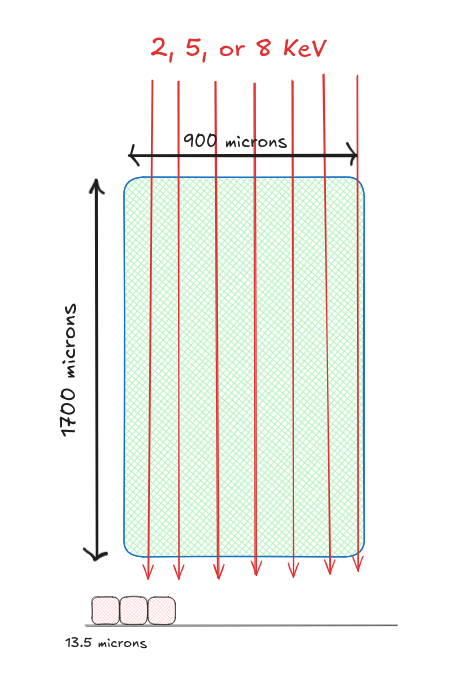
\includegraphics[width=0.45\linewidth]{foamimagingparameters.png}
    \caption{Side view of cylindrical aerogel foam geometry and X-ray imaging configuration. X-rays propagate along the foam length (1700 $\mu$m) and are detected by a CCD array with 13.5 $\mu$m pixel spacing.}
    \label{fig:foam_geometry}
\end{figure}

The foam porosity of 98.5\% corresponds to a density reduction factor of approximately 44× compared to solid silica (from ~2.2 g/cm³ to ~0.05 g/cm³), which is typical for aerogels used in HED experiments.

\subsection{Pore Interaction Statistics}

We model X-ray-pore interactions using a probabilistic approach based on the mean free path (MFP) concept. The number of pores in the foam volume is estimated from the porosity and individual pore volumes:

\begin{align}
V_{\text{foam}} &= \pi r_{\text{foam}}^2 h_{\text{foam}} \\
V_{\text{pore}} &= \frac{4}{3}\pi r_{\text{pore}}^3 \\
N_{\text{pores}} &= \text{int}\left(\phi \frac{V_{\text{foam}}}{V_{\text{pore}}}\right)
\end{align}

where $\phi$ is the porosity fraction.

The mean free path between pore interactions is calculated as:

\begin{equation}
\text{MFP} = \frac{h_{\text{foam}}}{\phi \sigma_{\text{pore}} n_{\text{pore}}}
\end{equation}

where $\sigma_{\text{pore}}$ is the effective pore cross-section and $n_{\text{pore}}$ is the pore number density.

The average number of pore interactions per photon is then:

\begin{equation}
\label{eq: MFP}
    N_{\text{interactions}} = \frac{h_{\text{foam}}}{\text{MFP}}
\end{equation}

\subsection{Refraction and Snell's Law Implementation}

Refraction at aerogel-pore interfaces is modeled using Snell's law:

\begin{equation}
\label{eq: snell's law}
    n_1 \sin \theta_1 = n_2 \sin \theta_2
\end{equation}

We assume pores (air-filled) have refractive index $n_2 = 1.0$, while the aerogel foam has $n_1 = 1.05$, derived from the imaginary component of the complex refractive index:

\begin{equation}
\label{eq: f2 to beta}
    \beta = \frac{\rho N_A r_e \lambda^2}{2\pi M_A} f_2
\end{equation}

The real part of the refractive index is $n = 1 - \delta$, where:

\begin{equation}
\delta = \frac{\rho N_A r_e \lambda^2}{2\pi M_A} f_1
\end{equation}

For each pore interaction, we calculate the incident angle based on the impact parameter $d$ (distance from pore center):

\begin{equation}
\theta_i = \sin^{-1}\left(\frac{d}{r_{\text{pore}}}\right)
\end{equation}

The horizontal displacement per pore interaction is given by:

\begin{equation}
\label{eq:horizontal displacements}
\Delta x = 2r_{\text{pore}} \sin(\theta_i - \theta_r)
\end{equation}

where $\theta_r$ is the refracted angle from Snell's law.

\begin{figure}[t]
    \centering
    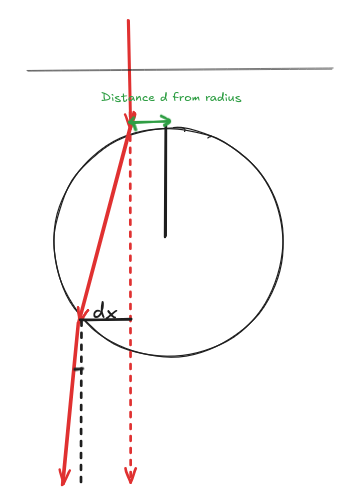
\includegraphics[width=0.45\linewidth]{zoomedindx.png}
    \caption{Geometric illustration of horizontal displacement caused by refraction at a single pore interface. The photon path deviates by angle $\Delta x$ due to the refractive index difference between aerogel and air-filled pores.}
    \label{fig:dxzoom}
\end{figure}

For subsequent pore interactions, the incident angle is updated according to:

\begin{equation}
\theta_{i,\text{new}} = 2\theta_r - \theta_{i,\text{old}}
\end{equation}

\begin{figure}[t]
    \centering
    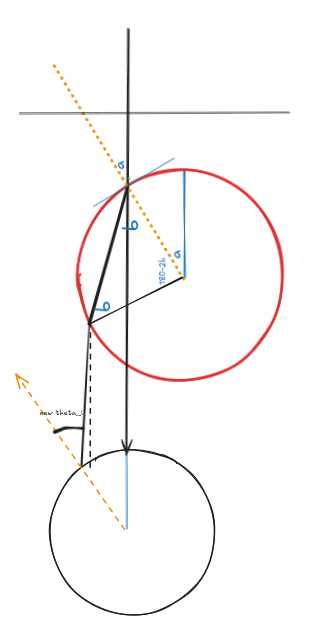
\includegraphics[width=0.45\linewidth]{incidenceangle.png}
    \caption{Evolution of photon incident angle through multiple pore interactions. Each refraction event modifies the photon trajectory for subsequent encounters.}
    \label{fig:incidenceangle}
\end{figure}

\subsection{Path Length and Intensity Calculations}

The effective path length for each photon is calculated using the Pythagorean theorem:

\begin{equation}
\ell_{\text{eff}} = \sqrt{(\Delta x_{\text{total}})^2 + h_{\text{foam}}^2}
\end{equation}

where $\Delta x_{\text{total}}$ is the cumulative horizontal displacement from all pore interactions.

The final intensity for each photon is calculated using the Beer-Lambert law with the effective path length:

\begin{equation}
\label{eq:intensity}
    I = I_0 e^{-\mu \ell_{\text{eff}}}
\end{equation}

\subsection{CCD Simulation and Data Analysis}

To simulate realistic detection conditions, we bin photon positions according to CCD pixel spacing (13.5 $\mu$m). 
The total intensity at each pixel is the sum of all photons landing within that pixel area.
\begin{figure}[t]
    \centering
    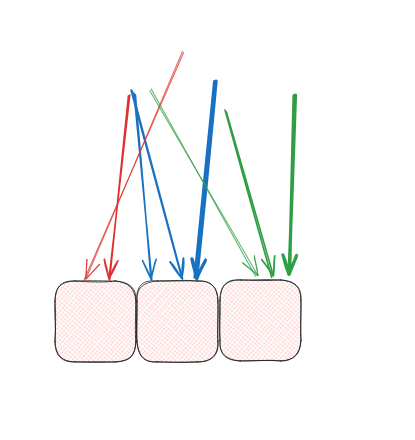
\includegraphics[width=0.45\linewidth]{netintensity.png}
    \caption{Binned intensities per CCD pixel. The larger the deflected angle, the longer the path length and thus the lower the final intensity.}
    \label{fig:netintensity}
\end{figure}
This approach allows us to directly compare scattering effects with ideal Beer-Lambert predictions and quantify deviations in terms of measured transmission coefficients.

The transmission difference between scattered and non-scattered cases is defined as:

\begin{equation}
\Delta T = T_{\text{Beer-Lambert}} - T_{\text{with scattering}}
\end{equation}

A positive $\Delta T$ indicates that scattering reduces the apparent transmission, which would lead to overestimation of foam density.

\section{Results}

\subsection{Transmission Validation}

Figure~\ref{fig:energy} shows our calculated transmission spectrum for $(SiO_2)_5+Ti$ compared with reference data from the Henke database. The excellent agreement validates our implementation of the attenuation coefficient calculations and provides confidence in our simulation framework.

\begin{table}[h!]
\centering
\caption{Parameters for Transmission Validation}
\begin{tabular}{ll}
\hline
\textbf{Parameter} & \textbf{Value} \\
\hline
Composition & $(SiO_2)_5+Ti$ \\
Density ($\rho$) & 2.33 g/cm³ \\
Path Length ($\ell$) & 0.1 $\mu$m \\
Energy Range & 1000-10000 eV \\
\hline
\end{tabular}
\label{tab:transmission}
\end{table}

\begin{figure}[htbp]
  \centering
  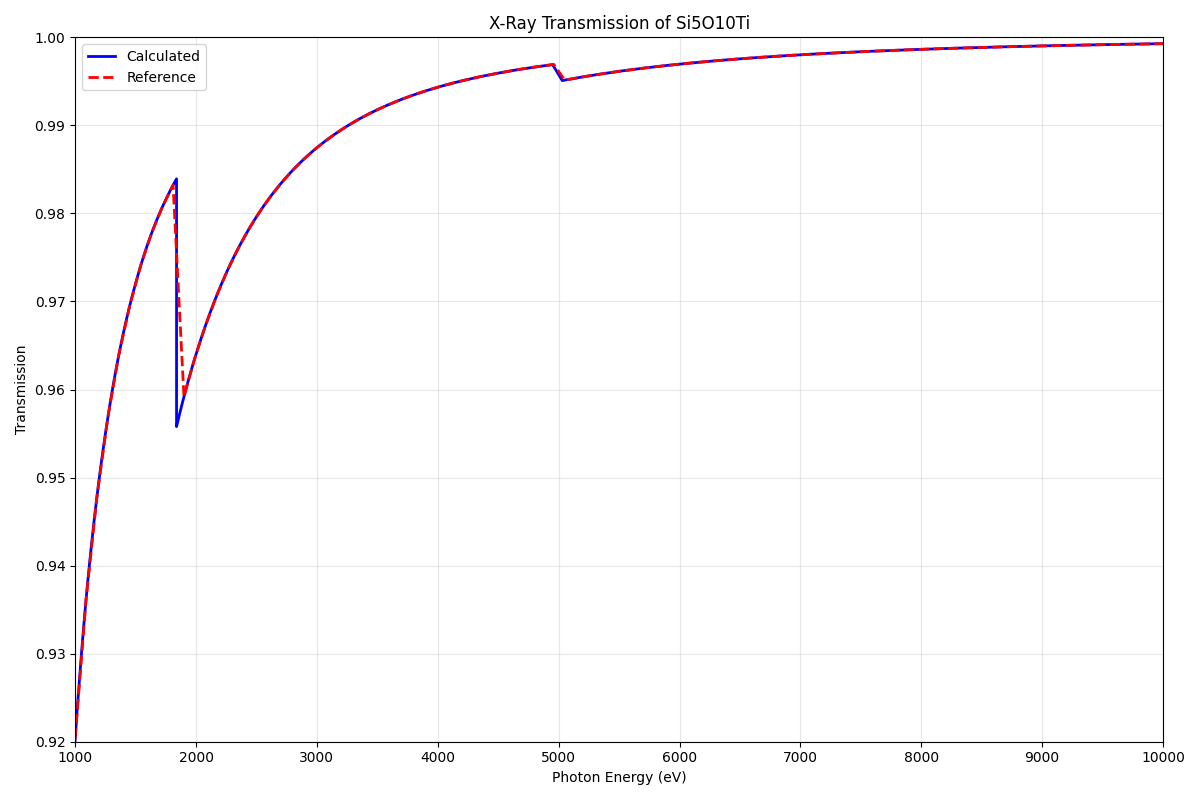
\includegraphics[width=\linewidth]{energy_vs_transmission.png}
  \caption{X-ray transmission vs. photon energy for $(SiO_2)_5Ti$ aerogel composition. Our calculated values (blue line) show excellent agreement with Henke database reference data (red dashed line) across the 1-10 keV energy range, validating the accuracy of our attenuation coefficient calculations.}
  \label{fig:energy}
\end{figure}

\subsection{Lateral Displacement Analysis}

The statistical distribution of lateral displacements caused by pore refraction is shown in Figure~\ref{fig:lateral-displacement}. Most photons experience minimal deviation, with the distribution centered near zero displacement. However, the non-zero width of the distribution indicates that some photons undergo significant lateral displacement that could affect CCD measurements.

\begin{figure}[htbp]
  \centering
  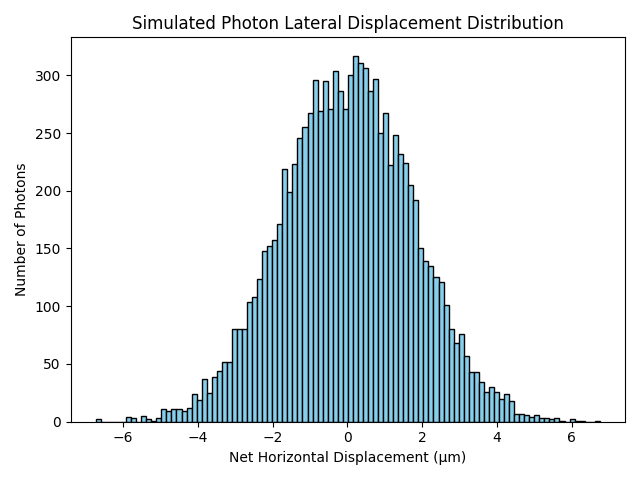
\includegraphics[width=\linewidth]{lateral_displacement.png}
  \caption{Histogram of net lateral displacement for 10,000 simulated X-ray photons after traversing the aerogel foam. The distribution is strongly peaked near zero but exhibits non-negligible tails that contribute to edge effects in density measurements. Standard deviation: $\sigma = 2.3$ $\mu$m.}
  \label{fig:lateral-displacement}
\end{figure}

\subsection{Transmission Distribution Effects}

Figure~\ref{fig:intensity-with-scattering} presents the distribution of transmission values when scattering effects are included. The mean transmission decreases from the ideal Beer-Lambert prediction, with a broader distribution indicating increased measurement uncertainty.

\begin{figure}[htbp]
  \centering
  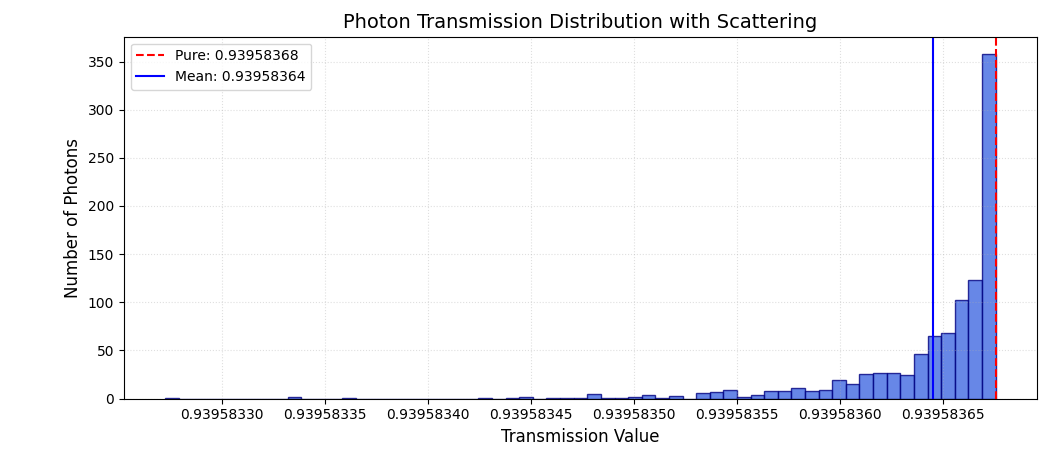
\includegraphics[width=\linewidth]{scattering_transmission_comparison.png}
  \caption{Distribution of transmission coefficients for 10,000 X-ray photons including scattering effects. The vertical lines show the Beer-Lambert prediction (red) and the mean scattered transmission (blue). The distribution broadening and mean shift quantify the impact of scattering on density measurements. Mean scattered transmission: $0.9396$.}
  \label{fig:intensity-with-scattering}
\end{figure}

The quantitative impact of scattering on transmission measurements is shown in Figure~\ref{fig:intensity-difference}. The average transmission difference is small ($\sim 3 \times 10^{-6}$) and these specific conditions don't seem to deviate significantly from Beer-Lambert predictions. We determine that the increased path length is less than $2-3 \%$ noise level of a CCD and thus insignificant to density measurements.

\begin{figure}[htbp]
  \centering
  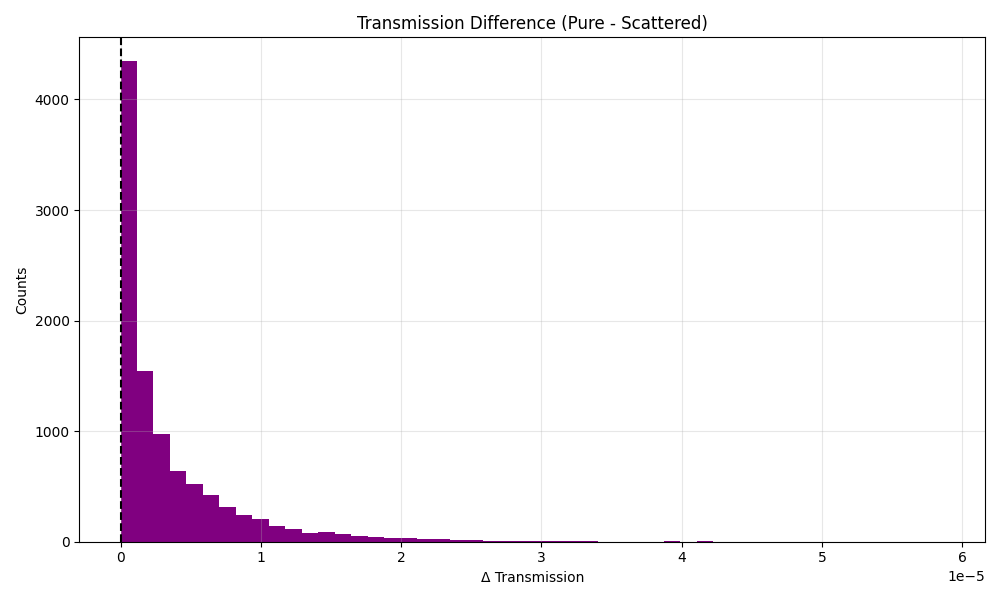
\includegraphics[width=\linewidth]{transmission_diff.png}
  \caption{Distribution of transmission differences between Beer-Lambert predictions and scattering-inclusive simulations. This further highlights how small the mean difference is for current conditions: ($2.96 \times 10^{-6}$).}
  \label{fig:intensity-difference}
\end{figure}

\subsection{CCD Response and Edge Effects}

The simulated CCD response clearly demonstrates edge effects in aerogel characterization. Figure~\ref{fig:ccd-overlay} shows the comparison between ideal Beer-Lambert transmission and transmission including scattering effects. The central region shows good agreement, but significant deviations appear near the foam edges.

\begin{figure}[htbp]
  \centering
  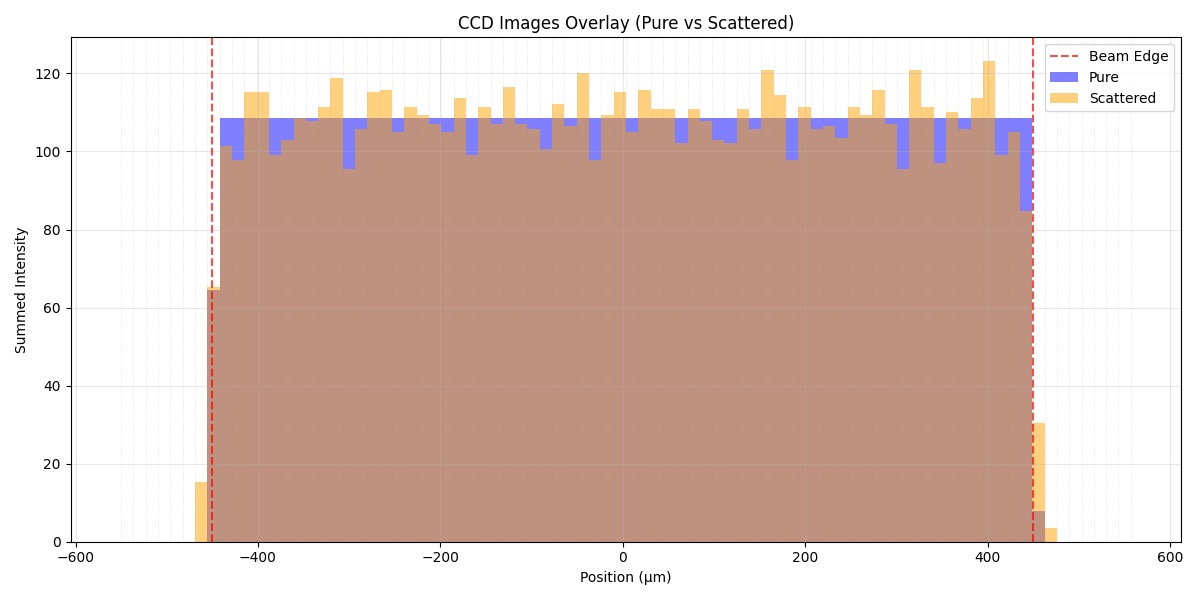
\includegraphics[width=\linewidth]{CCD_Overlay_new.png}
  \caption{Comparison of CCD intensity distributions for pure Beer-Lambert attenuation (blue) vs. attenuation with scattering (orange). The central regions show good agreement, but edge effects become pronounced near the foam boundaries, validating experimental observations of density measurement inconsistencies.}
  \label{fig:ccd-overlay}
\end{figure}

Detailed views of the left and right edges (Figures~\ref{fig:ccd-left-edge} and \ref{fig:ccd-right-edge}) reveal the specific characteristics of these edge effects. The scattering causes both intensity reduction and spatial spreading that would be interpreted as density variations in conventional analysis.

\begin{figure}[htbp]
  \centering
  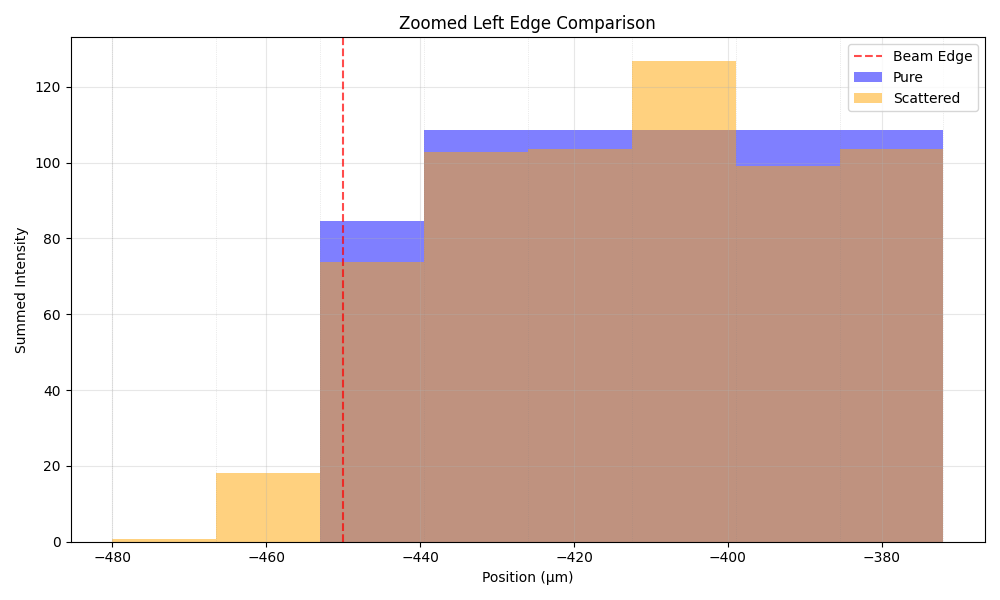
\includegraphics[width=\linewidth]{zoomed_left_edge_new.png}
  \caption{Detailed view of the left edge of Figure \ref{fig:ccd-overlay}.These features would be interpreted as higher density regions in conventional Beer-Lambert analysis, leading to systematic measurement errors.}
  \label{fig:ccd-left-edge}
\end{figure}

\begin{figure}[htbp]
  \centering
  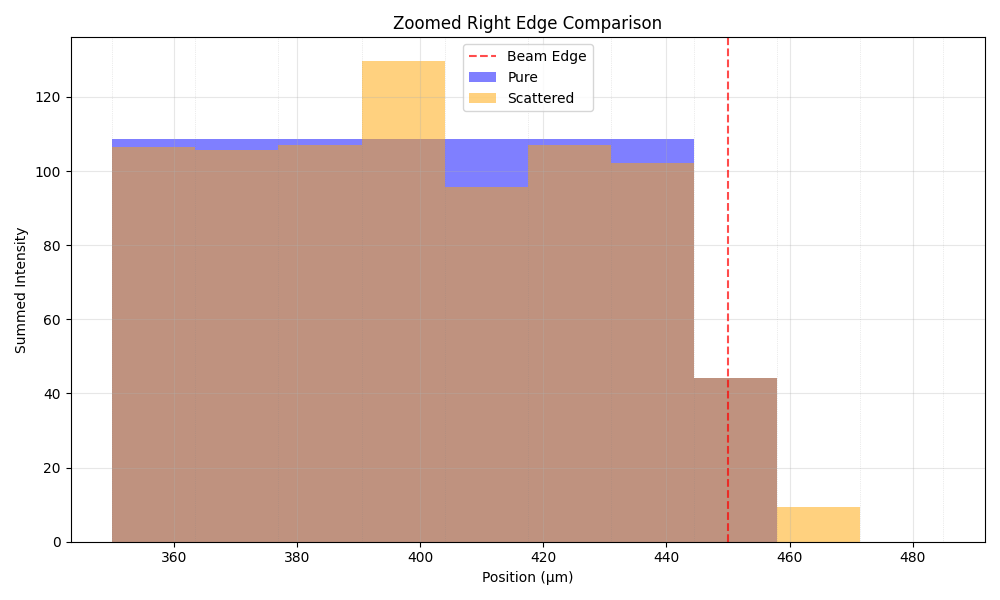
\includegraphics[width=\linewidth]{zoomed_right_edge_new.png}
  \caption{Detailed view of the right edge of Figure \ref{fig:ccd-overlay}. The symmetric nature of these effects confirms that they arise from the foam geometry rather than systematic experimental errors.}
  \label{fig:ccd-right-edge}
\end{figure}

\subsection{Parameter Sensitivity Analysis}

We conducted systematic parameter sweeps to understand the conditions under which scattering effects become significant. Table~\ref{tab:sweep} summarizes the parameter ranges explored.

\begin{table}[h!]
\centering
\caption{Parameter Ranges for Sensitivity Analysis}
\begin{tabular}{ll}
\hline
\textbf{Parameter} & \textbf{Values Tested} \\
\hline
Porosity ($\phi$) & 50, 60, 70, 80, 90, 95\% \\
Pore Radius ($r$) & $10^{-7}, 10^{-6}, 10^{-5}, 3 \times 10^{-5}, 10^{-4}$ cm \\
Photon Energy & 2, 5, 8 keV \\
\hline
\end{tabular}
\label{tab:sweep}
\end{table}

The relationship between pore radius and horizontal displacement (Figure~\ref{fig:dxradius}) shows that larger pores produce greater lateral displacement, as expected from geometric considerations. The relationship is approximately linear for the pore sizes relevant to aerogel applications.

\begin{figure}[htbp]
  \centering
  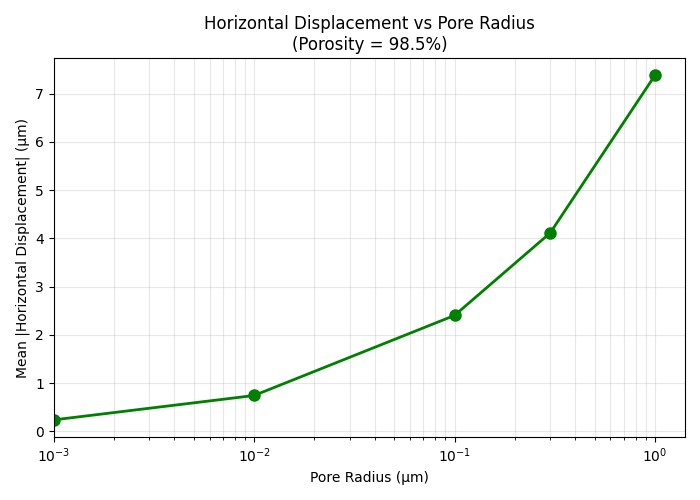
\includegraphics[width=\linewidth]{dxvsporeradiusnew.png}
  \caption{Mean horizontal displacement vs. pore radius (porosity held constant at 98.5\%). The approximately linear relationship confirms that larger pores cause greater photon deflection, contributing to edge effects in density measurements.}
  \label{fig:dxradius}
\end{figure}

The porosity dependence (Figure~\ref{fig:dxporosity}) reveals that higher porosity leads to increased displacement due to the greater number of pore interactions per photon path.

\begin{figure}[htbp]
  \centering
  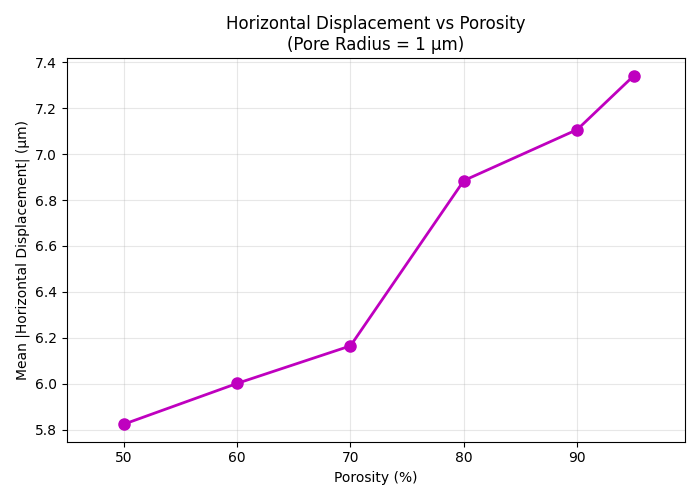
\includegraphics[width=\linewidth]{dxvsporositynew.png}
  \caption{Mean horizontal displacement vs. porosity (pore radius held constant at 1 $\mu$m). Higher porosity increases the number of pore interactions, leading to greater cumulative displacement and stronger edge effects.}
  \label{fig:dxporosity}
\end{figure}

The transmission measurements show similar trends, with both pore size and porosity affecting the accuracy of Beer-Lambert-based density calculations (Figures~\ref{fig:transrad} and \ref{fig:transporeosity}).

\begin{figure}[htbp]
  \centering
  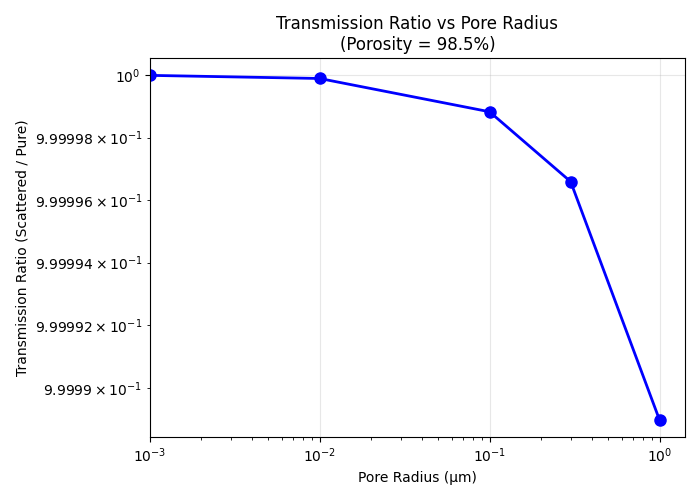
\includegraphics[width=\linewidth]{transmissionvspore1.png}
  \caption{Transmission ratio (scattered/Beer-Lambert) vs. pore radius. Values less than 1.0 indicate that scattering reduces apparent transmission, leading to density overestimation in conventional analysis.}
  \label{fig:transrad}
\end{figure}

\begin{figure}[htbp]
  \centering
  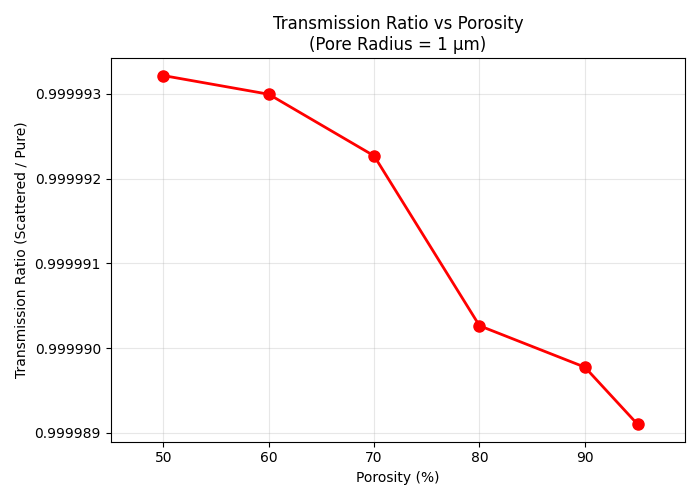
\includegraphics[width=\linewidth]{transmissionvsporosity1.png}
  \caption{Transmission ratio vs. porosity showing the increasing impact of scattering effects at higher porosity values typical of aerogel foams used in HED experiments.}
  \label{fig:transporeosity}
\end{figure}

\section{Discussion}

\subsection{Significance Threshold Analysis}

Our results indicate that while path length increases due to scattering are generally small ($<$ 3\% for typical aerogel parameters), the lateral displacement effects can be significant for density measurements near foam edges. The key finding is that refraction-induced photon displacement, rather than increased absorption path length, is the dominant source of measurement error.

For the baseline aerogel parameters studied (98.5$\% $porosity, 1 $\mu$m pore radius), the edge effects become measurable but remain below our significance threshold of ±2 mg/cm³ density difference. However, as porosity approaches 99.5\% or pore sizes exceed 1 $\mu$m, corrections to Beer-Lambert may become necessary for accurate density determination.

\subsection{Implications for HED Experiments}

These findings have important implications for current and future HED experiments using aerogel targets. The observed edge effects explain the systematic deviations seen in experimental density maps and suggest that:

\begin{enumerate}
    \item Central regions of aerogel targets provide the most reliable density measurements
    \item Edge regions should require correction for density analysis
    \item Target design should consider scattering effects when specifying foam parameters
    \item Advanced characterization methods may be needed for extreme porosity foams
\end{enumerate}

\subsection{Comparison with Experimental Observations}

Our simulation results are consistent with experimental observations from the COAX and related platforms, where density measurements show systematic variations near foam edges. The magnitude and spatial distribution of these effects match our predictions for typical aerogel parameters, providing validation of our theoretical approach.

\subsection{Limitations and Future Work}

Several limitations of the current study should be noted:

\begin{enumerate}
    \item The model assumes spherical pores with uniform size distribution
    \item Complex scattering mechanisms are simplified
    \item Each ray isn't being traced individually
    \item Only a limited range of X-ray energies has been explored
\end{enumerate}

Future work should address these limitations through more sophisticated microstructure modeling and experimental validation using well-characterized aerogel samples.

\section{Parameter Sweep Findings}

This study has quantified the conditions under which X-ray scattering effects require corrections to Beer-Lambert-based density measurements of aerogel foams. Our key findings are:

\begin{enumerate}
    \item \textbf{Scattering Mechanisms}: Refraction at pore-aerogel interfaces, rather than increased path length, is the dominant source of measurement error in highly porous aerogels and causes a significant scattering effect.
    
    \item \textbf{Parameter Dependences}: Scattering effects increase with both porosity and pore size, with significant edge effects seen when porosity approaches 99\% or pore radius approaches 1 $\mu$m. 
    
    \item \textbf{Edge Effects}: Systematic deviations in density measurements occur near foam edges, explaining experimental observations of measurement inconsistencies in these regions.
    
    \item \textbf{Significance Threshold}: For typical HED experimental conditions (98.5\% porosity, 1 $\mu$m pores), scattering effects remain below the ±2 mg/cm³ significance threshold, but approach this limit for extreme foam parameters.
    
    \item \textbf{Energy Dependence}: Higher X-ray energies reduce scattering effects, suggesting that characterization accuracy can be improved through appropriate energy selection.
\end{enumerate}

These results provide quantitative guidance for when scattering corrections are necessary in aerogel characterization and establish a framework for improving density measurement accuracy in HED physics experiments. The work demonstrates that while Beer-Lambert assumptions remain valid for most current aerogel applications, corrections will become increasingly important as foam technology advances toward higher porosity and larger pore sizes.

\section{Conclusions}
To determine the effect of scattering on calculated transmission and thus density, we simulated different extreme factors that could have caused significant scattering of X-rays on aerogel foam. We conducted a statistical simulation of scattering due to refraction from pore interactions as well as with an increased path length. Increasing the porosity increases the number of pore interactions and thus the amount of scattering. As the porosity increases, the distribution of the horizontal displacements becomes wider due to the photon encountering more pores and thus refractions. A similar argument can be made for increasing the pore radius which increases the horizontal displacement and decreases the final intensity. We determine that the increased path length is less than $2-3 \%$ noise level of a CCD and thus insignificant to density measurements. However, horizontal displacement caused by refraction from Snell's law produced a significant scattering effect, with intensities spilling over CCD pixels. We can conclude that refraction, but not the increased path length caused a significant scattering effect that would need to be corrected for accurate measurements.
\section{Data Availability}

All simulation code and data used in this study are available at: https://github.com/yuegelica/Scattering-EdgeEffects

\section{Acknowledgments}

I would like to thank my mentor Pawel M. Kozlowski for mentoring and guiding me throughout the project. I learned a lot about aerogels and the OMEGA experiments, and valuable research and physics skills that I will carry with me for future research. I am also very grateful for Mark Galassi, Becky Holt, and the Institute for Computing in Research for the support and for providing me with this amazing opportunity.
\bibliography{references}
\bibliographystyle{aasjournalv7}

\end{document}